\documentclass{article}

% if you need to pass options to natbib, use, e.g.:
% \PassOptionsToPackage{numbers, compress}{natbib}
% before loading nips_2016
%
% to avoid loading the natbib package, add option nonatbib:
% \usepackage[nonatbib]{nips_2016}

% \usepackage{nips_2016}

% to compile a camera-ready version, add the [final] option, e.g.:
\usepackage[final]{nips_2016}

\usepackage[utf8]{inputenc} % allow utf-8 input
\usepackage[T1]{fontenc}    % use 8-bit T1 fonts
\usepackage{hyperref}       % hyperlinks
\usepackage{url}            % simple URL typesetting
\usepackage{booktabs}       % professional-quality tables
\usepackage{amsfonts}       % blackboard math symbols
\usepackage{nicefrac}       % compact symbols for 1/2, etc.
\usepackage{microtype}      % microtypography
\usepackage[pdftex]{graphicx}
\usepackage{subfigure}

\title{Lat-Net: Compressing Lattice Boltzmann Fluid Simulations using Deep Neural Networks}

% The \author macro works with any number of authors. There are two
% commands used to separate the names and addresses of multiple
% authors: \And and \AND.
%
% Using \And between authors leaves it to LaTeX to determine where to
% break the lines. Using \AND forces a line break at that point. So,
% if LaTeX puts 3 of 4 authors names on the first line, and the last
% on the second line, try using \AND instead of \And before the third
% author name.

\author{
  Oliver Hennigh \\
  Mexico \\
  \texttt{loliverhennigh101@gmail.com} \\
}

\begin{document}
% \nipsfinalcopy is no longer used

\maketitle

\begin{abstract}
We present Lat-Net, a method for compressing both the computation time and memory usage of lattice boltzmann flow simulations using deep neural networks. Lat-Net employs convolutional autoencoders and residual connections in a fully differentiable scheme to compress the state size of a simulation and learn the dynamics on this compressed form. The result is a small computationaly and memory effecient neural network that can be itereated and queired to reproduce a fluid simulation. While we apply Lat-Net to fluid simulations   and in addition to applying it to both 2d an 3d fluid flow simulations, we also show it can be used  computed with the Lattice Boltzmann method. We also show that by training on small scale simulations we can use the learned network to generated larger simulations accuratly.

\end{abstract}

\section{Introduction}

(breif high level paragraph)

Computational fluid dynamics (CFD) is a branch of fluid dynamcis that deals with numericaly solving and analyzing fluid flow problems such as those found in aerodynaics, geological morphol, and biomedical. CFD simulations are known for their high computational requirements, memory usage, and run times. Becuase of this, there is an ever growing body of work on using simulation data to create surrogate or metamodels that can be evaluated with sigificantly less resources. Towards this end, we develop a neural network approach that both compresses the computation time and memory usage of fluid simulations.

(Talk about type of fluid simulations)

There are many different types of fluid flow . In particlular, we investigate fluid simulations that contain complex time dependet phenomena such as vortexs. Simulations of this form are difficult because they require fluid solver to have high resolution and small times steps. Never the less, they are very important for studing things like blaa. Motivated by need for these simulations and the suscess of neural network based suraget models in related areas, we choice this setting to test our model (bad wording).

(Say that we are using LBM and why)

The most popular approach to modeling fluid flow is with the Navier stokes equation. This partial differential equations (blaa). Relativily recently there has been a new method for solving fluid flow named the Lattice Boltzmann Method. It is derived from . The main advantage of LBM is its ability to run on massibely parallel architectures. Because of this there has been much development in the area. Because of this methods popularity and techinqual details we will go over later, our approach is centered around this method of simulation.

(give breif description of method)

Our proposed method works by compressing state of the simulation while learning the dynamics of the simulation on these compressed forms. The model can be broken up into three pieces, an encoder, compression mapping, and decoder. The encoder compresses the both the velocity and density vector field as well as the given boundary conditions to a compressed form. The compression mapping learns mappings on the compressed state while applying boundary conditions that corrispond to the time steps in the fluid simulation. The decoder decompresses the compressed state allowing for either the whole velocity and density vecotr field to be extracted or desired measurments.

(Say that we also look at Electormagnetic simulations)

We focus the content of this paper on LBM Fluid Simulations because this is the most popular use of LBM however LBM is known to be a general partial differential equation solver (of a particular form cite em paper). LBM can in fact be used to solve many physical systems of interest such as Electormagnatism, Plasma, Multiphase flow, Schordiener equation etc. (find good citations for all of these). With this in mind we keep our method general and show evidence our method works equaly effectively on Electromagnatism simulations. However, Because the domanate use of LBM is on fluid flow problems we center discustion on this subject with only minor look at other problems

(List the contirbutions concisly)

Our method has several key contributions over other work creating surage models of fluid simulations with neural networks. First, It allows for simulations to be generated with an order of magnatude less memory. There is a crucial need for such suragat models because memory requirements grow cubic to grid size in 3d simulations. In practice this quickly results in the need for supercomputers (tokyo stuff)(bad wording). Second, once our model is trained it can be used to generate significantly larger simulations. This allows the model to learn from a large training set of small simulations and then generate simulations as much as 16 times bigger with little effect in accuracy. Third, our method is directly applicable to a variety of physics simulations, not just fluid flow.

(Maybe Talk about the need for better flow solvers)

As the high performance computing (HPC) is expanding, computational fluid dynamics faces numerous chalanges in makeing 


\section{Related Work}

Recently, there have been several papers applying neural network to fluid flow problems. Xiaoxiao etc \cite{guo2016convolutional} proposed to use a neural network to learn a mapping from the boundary conditions to the steady state flow. In China guy paper, noone knows what they did because there is no way to get the paper. Most related to our own work, Tompson ect. \cite{tompson2016accelerating} uses a network to solve the (blaa) to accelerate eulerian fluid simulations. The key difference between this and our proposal is the ability to compresse the memory and the generability of our method.

There

Our model is closely related to many video prediction works. Video prediction is the problem of generated future frames in in video data given previous frams. There is a ever growing body of work using neural networks to achevie this. To our knoweledge the first used recurrent temporal restricted Boltzmann machine (RTRBM) to model videos of bouncing balls (we also look at this problem). There have also been recurrent grammar cells applied to varieous time seires tasks including bouncing balls and NORBvideos. More recently there is lots of work in video prediction for application to rienforcment learning and control. These models use a variety of techniques for next frame prediction such as straight convolutions  to LSMTs. (need to put video cnn in here).

(Reduced order modeling)

\section{Deep Neural Networks for Compressed Lattice Boltzmann}

In this section, we present our model for compressing Lattice Bolztmann simulation.

\subsection{Review: The Lattice Boltzmann Method}

As mentioned above, our method is centered around the LBM. There are several key reasons for doing this but discusing them requires a breif overview of the LBM. While there are many variations of the method we will only discus LBM simulations with the BGKD collision operator. 

(high level overview of method)

The Lattice Boltzmann Method has been developled relatively recently having evolved from the Lattice Gas Automata in the 90s. It has a fundamentaly different approach to modeling fluid then typical PDE approaches. While there are a variety of ways to derive and view the LBM, the simplest discritption is that it models fluid with cells containing a flow flow distrobutions. These cells are updated 

(talk more specific about collision operator and e)

The Lattice Boltzmann algorithm comes down to the 

(Maybe not put this here)
(Why this is important)

The important aspect of the LBM for our purposes is that it acts localy on grid cells. The area of effect a cell is directly proporitional to the number of applications of the evolution equation. This means that in $n$ time steps a cells value can be determinied exaclty with only the infomation of the cells within $n$ distance. This is important to know for our purposes becasue if we expect to treat the lattice boltzmann simulation as deterministic we must make sure our model 

\begin{itemize}
  \item LBM is used in huge simulations
  \item LBM is very memory intensive
  \item LBM acts localy
  \item LBM can be implemented with 3x3 convs
  \item explain why this is important
\end{itemize}

\subsection{Proposed Architecture}

\begin{figure}[!t]
\centering
\subfigure{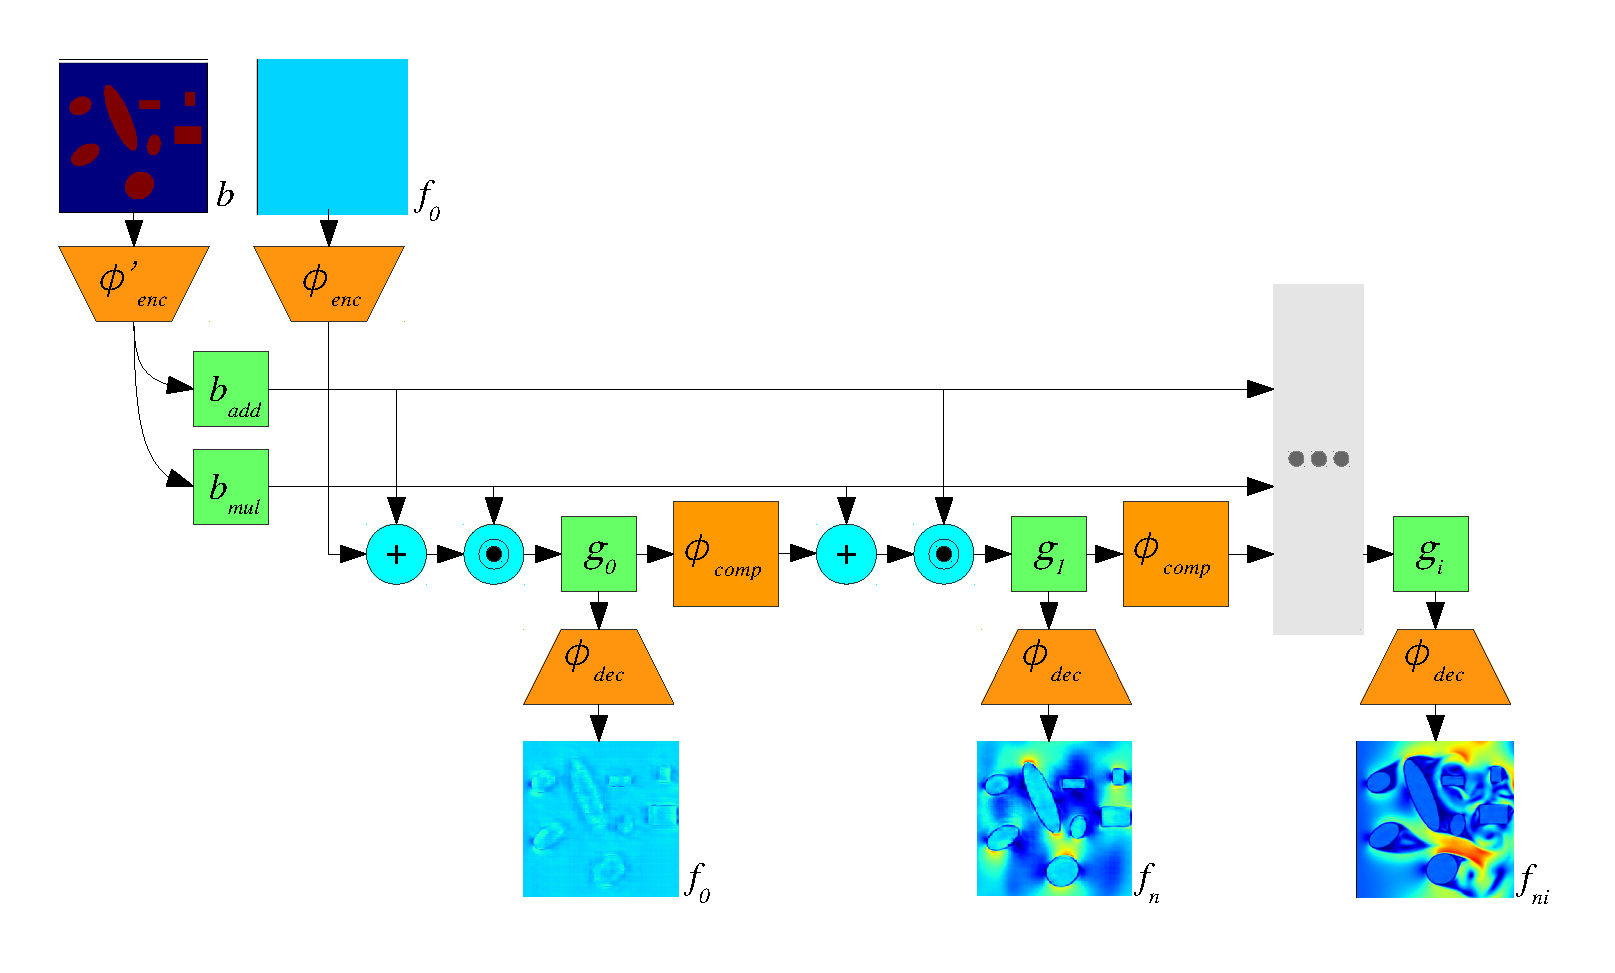
\includegraphics[scale=0.3]{../test/figs/fig_1.pdf}}
\caption{Lat-Net architeture }
\label{fig_1}
\end{figure}

Figure \cite{fig_1} shows a general scetch of the model. The figure can be understood by following the arrows starting from the flow state $f_t$ and the boundary $b$. Bellow we walk through each step of our method.

First the network compresses both the state of the fluid simulation $f_t$ and a binary representation of the boundary conditions $b$ using two seperate neural networks $\phi_{enc}$ and $\phi'_{enc}$ respectively. The result from $\phi_{enc}$ is a compressed representation of the flow $g_t$ and the result of $\phi'_{enc}$ are two tensors $b_{mul}$ and $b_{add}$ of equal size to $g_t$. These three tensors represent the entirety of the compressed state of the simulation.

In a lattice boltzmann solver the boundary conditions are used at each timestep to modify the propogation operator. In a similar way, our model applies the compressed boundary conditions to the compressed state every timestep. We do this in the following way,
\begin{equation}
  g_t = (g_t \odot b_{mul}) + b_{add}
\end{equation}
This method has proved extremely succesfull at keeping the boundary firmly planted through the diration of the simulation. This method of applying boundary conditions was inspired by\cite{vondrick2016generating} where they use a similar method to combine forground and background imformation in video prediction.

One timestep of the LBM is
After the boundary is applied to $g_t$ we can run the state through another neural network to emulate the dynamics, $\phi_{comp}$. 

After $g_t$ is computed we can extract out the generated state of the simulation with a decoder network $\phi_{dec}$. 

\subsection{Network Implementation}

(go over why the network is kept convolutional)

As mentioned above, each network is kept entirley convolutional. This allows spatial information to be preserved. During the course of this work, fully connected layers were explored for use in the compression mapping however this produce extremely poor results.

(go over importance of residual connections)

Residual connections have been used in many machine learning tasks with much sucess. Adding redidual connections allows for much deeper networks to be trained often resulting in improved results. When training our model it is necesarry to unroll the compression network over several time steps. This has the same effect as making the network deeper when training. For this reason it seems advantagouse to take advantage of this network architecture. We have seen that removing removing these conections results in much slower convergence and worse accuracy.

Down sampling is produced by 4 by 4 convolutions with stride 2. Some of the simulations trained on have periodic boundary conditions. In these cases, we pad the opropriot edges periodicily before the convolution operations.


\subsection{Training Details}

Lat-Net is trained with the Adam optimizer. 
Our loss function is a combination of Mean Squared Error (MSE) and Image Gradient Difference Loss (GDL)\cite{mathieu2015deep}.

\subsection{Electromagnetic Simulations}

The LBM with the 

\section{Experiments}

In this section we descirbe our experiments testting Lat-Net on a variety of problems. Our experiments are designed to tests our models ability to generate large simulations as well as the trade of between memory compression and error. We also give results on the computational speed increase and its effectiveness at generating Electormagnetic Simulations.

\subsection{Dataset Generation}
In order to train and test our model, we generated sets of fluid and electromagnetic simulations.

The train set for the 2 dimensional fluid simulation are grid size 256 by 256 and use 9 directional flows in the lattice boltzmann solver (D2Q9 scheme). The simulation used periocid boundary conditions on top and bottom as well as uniform inlet flow and outlet flow of 0.04 from the left and right. 8 Objects are placed randomly with height and width sizes rangeing from 140 to 20 cells. The test set for the 2 dimesional simulations are of size 256, 512, and 1024. The same left, right, top and bottom boundary conditions are used with the number of objects being placed 8, 32, 128 respective to the size of the simulation. 

The train set for the 3 dimensional fluid simulations are grid size 40 by 40 by 160 and use 15 directional flows in the lattice boltzmann solver (D3Q15 scheme). Similar to the 2d simulations, periodic boundary conditions are used with same inlet and outlet flow. 4 spheres are randomly placed with height and width 24. The reason different object geometrys and sizes were not explored was due to the fact that smaller objects or objects with complex geometries tended to have too course a resolution for the lattice boltzmann solver and larger objects required too large a simulation size. The test set comprises (not sure yet).

(em dataset)

\subsection{Generating Large Simulation}



\begin{figure}[!t]
\centering
\subfigure{\includegraphics[scale=0.9]{../test/figs/256x256_2d_flow_image.png}}
\subfigure{\includegraphics[scale=0.9]{../test/figs/1024x1024_2d_flow_image.png}}
\caption{Accuracy of 2d fluid simulations }
\label{fig:bouncing_balls_error_3}
\end{figure}
\begin{figure}[!t]
\centering
\subfigure{\includegraphics[scale=0.3]{../test/figs/256x256_2d_error_plot.png}}
\subfigure{\includegraphics[scale=0.3]{../test/figs/1024x1024_2d_error_plot.png}}
\caption{Accuracy of 2d fluid simulations }
\label{fig:bouncing_balls_error_3}
\end{figure}

The force is calculated with the momentum transfer method \cite{guo2013lattice}

\subsection{Memory Compression and Effect on Error}
\begin{figure}[!t]
\centering
\includegraphics[scale=0.3]{../test/figs/compression_error_plot.png}
\caption{The effecto of Compression on MSE}
\label{}
\end{figure}

One of purposes of Lat-Net is to be able to compress the memory usage of large simulations and so it is a natural question to ask what effect the compression has on error. The ideal method to test this would be to train many models and compare their accuracy. Unforcunatly training models is extremely computational intensive and so we propose another approach. We instead train $\phi_{enc}$ and $\phi_{dec}$ in an autoencoder fassion and then measure the reconsturction MSE on the test set. This less computationaly expensive approach allows many models to be trained and evaluated.

By keeping the architeture of $\phi_{enc}$ and $\phi_{dec}$ the same and vareing the final compressed filter size we see the trade off between compression and error. It is interesting to see a diminising return effect for low compression ratios.

\subsection{Computational Speed Up}

Lattice Bolztmann Compression 

\begin{table}[]
\caption{Computation time of Networks peices} \label{compute_times}
\centering
\begin{tabular}{|l|lllll|}
\hline
Simulation    & Compression Mapping & Full State  & Plane      & Line       & Point   \\ \hline
(1024, 1024)  & 1.042 ms            & 15.832 ms   & na         & 2.647 ms   & 2.490 ms \\ 
(80, 80, 320) & 13.819 ms           & 127.553 ms  & 30.860 ms  & 18.457 ms  & 14.392 ms \\ 
\hline
\end{tabular}
\end{table}

\subsection{Electromagnetic Results}



\begin{figure}[!t]
\centering
\subfigure{\includegraphics[scale=0.9]{../test/figs/256x256_2d_em_image.png}}
\subfigure{\includegraphics[scale=0.9]{../test/figs/512x512_2d_em_image.png}}
\caption{Accuracy of 2d fluid simulations }
\label{fig:bouncing_balls_error_3}
\end{figure}
\begin{figure}[!t]
\centering
\subfigure{\includegraphics[scale=0.3]{../test/figs/256x256_2d_em_error_plot.png}}
%\subfigure{\includegraphics[scale=0.9]{../test/figs/512x512_2d_em_error_plot.png}}
\subfigure{\includegraphics[scale=0.3]{../test/figs/256x256_2d_em_error_plot.png}}
\caption{Accuracy of 2d fluid simulations }
\label{fig:bouncing_balls_error_3}
\end{figure}


\section{Conclusion}

Fluid Simulations are increadbly important for a variety of tasks however they are extreamely computation and memory intensive. In this work we have developed a unique method to tackle this problems using deep neural networks. We have demonstrated it is capable of accuratly reconstructing a variety of simulations under different conditions. We have also shown that our method can be readly applied problems other then flow.

The main limitation in our current model is blaa and. Future imporvements 

\begin{itemize}
  \item future work, customized loss
\end{itemize}

\section*{References}

\bibliography{references}
\bibliographystyle{ieeetr}

\end{document}
